\section{Methodology}
\label{sec:methodology}

\subsection{Research Design}

This study develops and validates an object-level metric for partial LiDAR visibility. The metric is intended to quantify the proportion of a labelled object that is observable from a specified sensor viewpoint. It is therefore distinguished from detector accuracy and from broader measures of point-cloud quality. Range, angular sampling, point density, and detector architecture may affect perception outcomes, but they are treated as covariates or comparison baselines rather than as definitions of occlusion.

The primary experiments will use the Mixed Signals V2X dataset because it provides synchronised observations from vehicles and roadside infrastructure. Each sensor--object pair will be treated as a separate observation, allowing the same object to be compared from viewpoints with different levels of occlusion.

\subsection{Experimental Pipeline}

\begin{figure}[H]
    \centering
    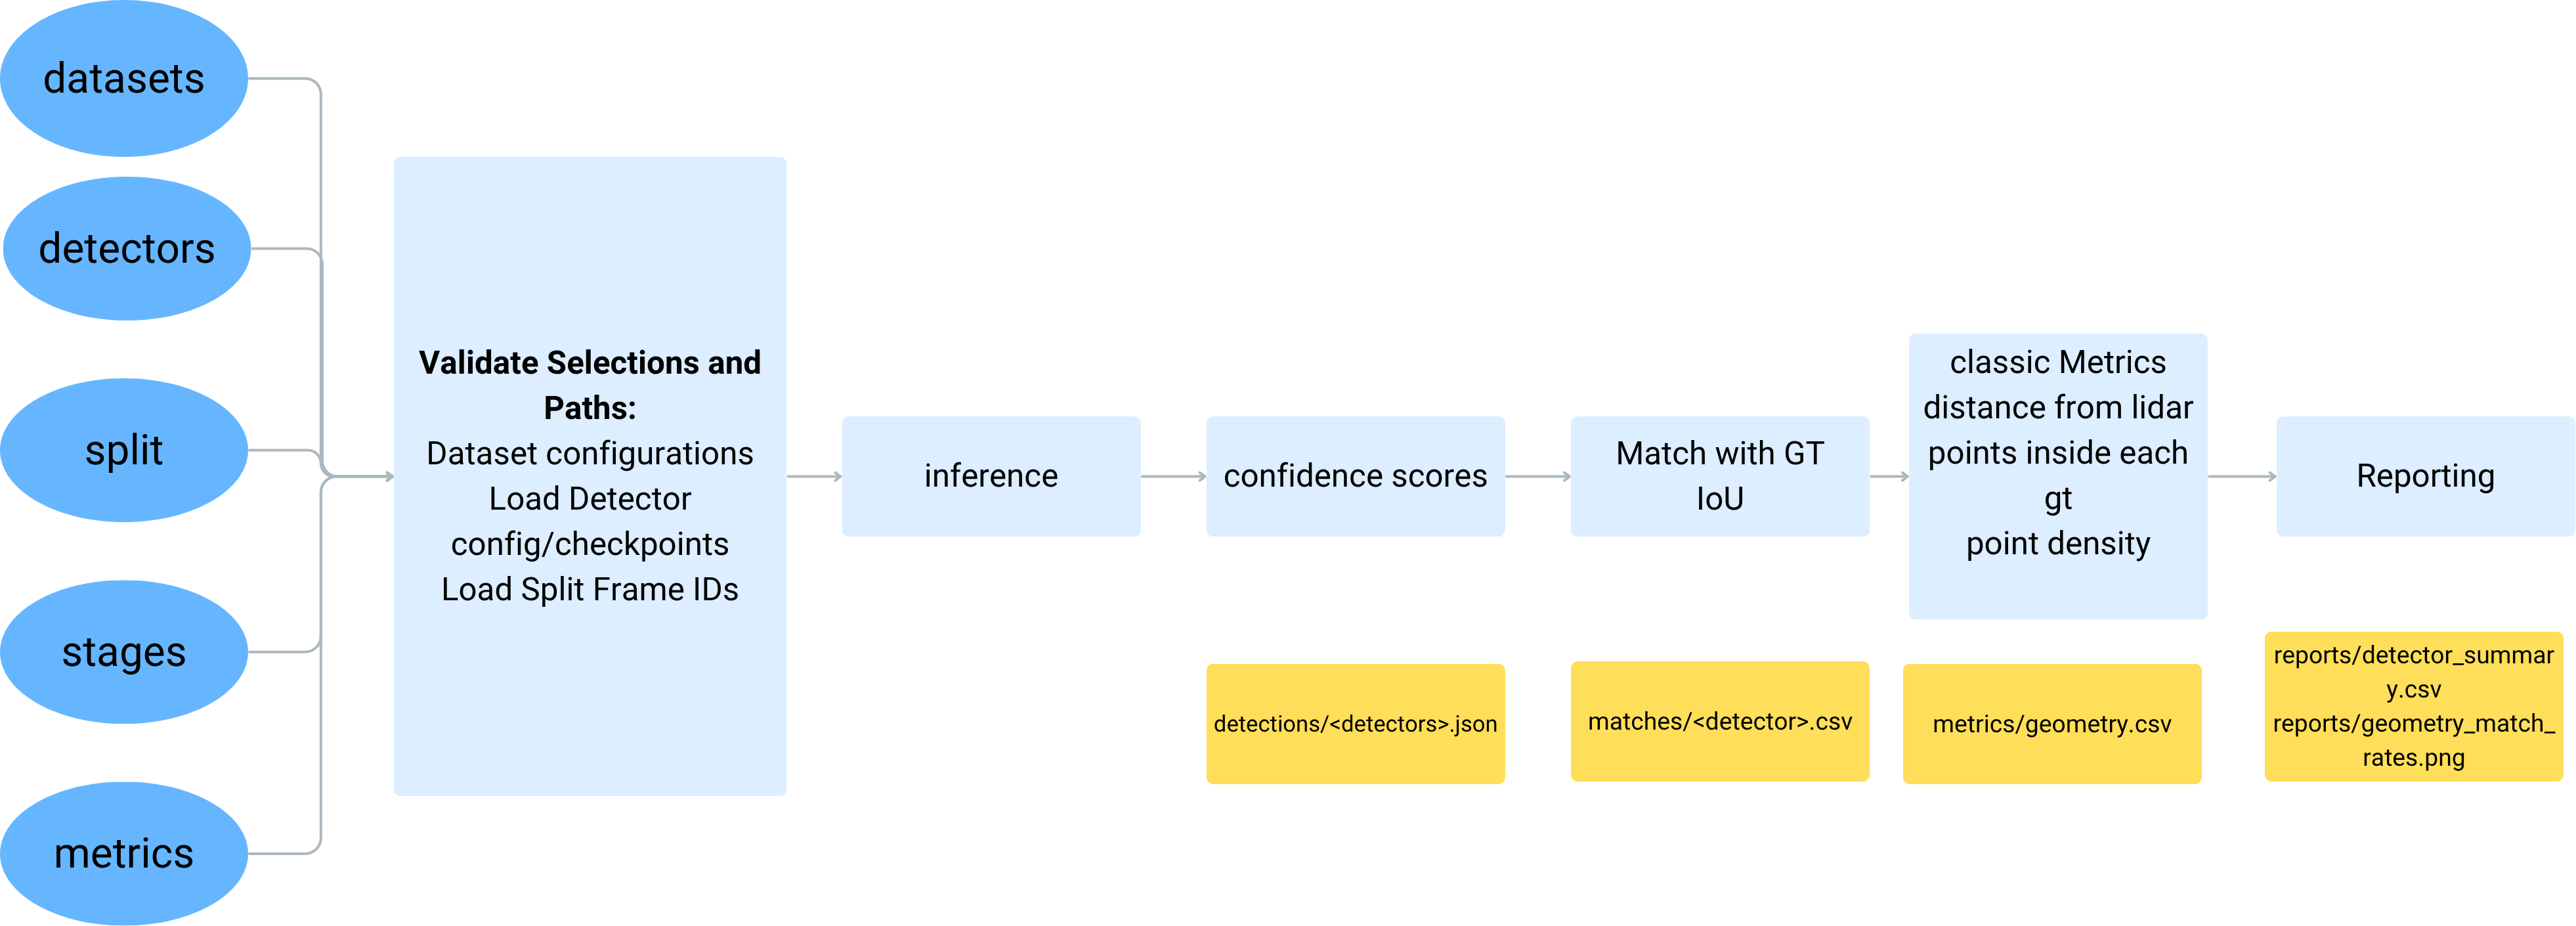
\includegraphics[width=\linewidth]{images/thesis-flow1.png}
    \caption{Proposed experimental pipeline for metric development and validation.}
    \label{fig:classic-pipeline}
\end{figure}

As shown in Figure~\ref{fig:classic-pipeline}, the pipeline comprises dataset preparation, baseline detector evaluation, occlusion-metric computation, and statistical validation. Dataset versions, coordinate transformations, class mappings, train--validation splits, preprocessing settings, detector configurations, and metric definitions will be recorded to support reproducibility.

\subsection{Dataset Preparation}

For every labelled object, LiDAR returns within the corresponding ground-truth 3D bounding box will be extracted and transformed into a common object-centred coordinate frame. The processing stage will retain the sensor pose, object pose, range, azimuth, object dimensions, class label, point count, and source agent. Quality checks will identify empty boxes, annotation inconsistencies, temporal misalignment, and points that lie close to bounding-box boundaries.

To prevent information leakage, detector selection and metric calibration will use the training partition, hyperparameter choices will use the validation partition, and final results will be reported on a held-out test partition where the dataset permits.

\subsection{Object-Level Visibility Metric}

Let $S_i$ denote the surface of object $i$ that would be observable from a sensor viewpoint in the absence of external occluders, and let $V_i \subseteq S_i$ denote the portion that remains visible after line-of-sight obstruction. The proposed visibility score is

\begin{equation}
    v_i = \frac{A(V_i)}{A(S_i)},
    \qquad 0 \leq v_i \leq 1,
\end{equation}

where $A(\cdot)$ is surface area. The corresponding occlusion score is $o_i = 1-v_i$, so larger values indicate greater occlusion.

Visibility will be estimated by ray tracing from the relevant LiDAR origin towards sampled points on the object surface. A sample is classified as externally occluded when another labelled object or reconstructed scene surface intersects the ray before the target. Surfaces facing away from the sensor will be handled separately as self-occlusion. Reporting external occlusion and self-occlusion separately will prevent two geometrically different phenomena from being hidden inside a single score.

Because observed returns also depend on range, beam pattern, incidence angle, reflectivity, and weather, raw point count and point density will not be included directly in the definition of $o_i$. Instead, they will be reported as baseline observability measures and used as covariates during validation. If sufficiently accurate surface models are unavailable, a bounding-box surface approximation will be used and documented as a limitation.

\subsection{Baseline Detector Pipeline}

A reproducible baseline will be established using an off-the-shelf LiDAR 3D object detector, such as PointPillars or SECOND, selected according to dataset compatibility and the availability of suitable pretrained weights. The detector will be evaluated using the dataset's standard protocol. Aggregate results will include precision, recall, F1-score, intersection over union (IoU), and mean average precision (mAP), where applicable.

Per-object outputs will include detection status, confidence, and localisation error. The same dataset partitions, annotation conversions, class mappings, and preprocessing steps will be used across experiments. Any unavoidable departure from an original implementation or benchmark setting will be documented explicitly.

\subsection{Validation and Statistical Analysis}

Construct validity will be assessed by testing whether increasing occlusion is associated with poorer detector outcomes. Analyses will compare the proposed score with point count, point density, range, and existing categorical difficulty labels. Detection status will be analysed using logistic regression, while confidence and localisation error will be examined using appropriate correlation or regression models. Range, object class, object size, source agent, and point density will be included as covariates where supported by the sample size.

Performance will also be reported in score bins to show whether detector degradation is monotonic. Bootstrap confidence intervals will be used to quantify uncertainty. Sensitivity analyses will examine the effects of surface-sampling resolution, bounding-box approximation, ray-intersection tolerance, and the treatment of self-occlusion.


The validation design adapts the fine-grained stratification used by Gilroy et al. for image-based pedestrian detection \cite{bib_ref_32}. Rather than reproducing their two-dimensional body-area metric or assuming that image-domain detector rankings transfer to LiDAR, the proposed continuous visibility score will be divided into sufficiently populated intervals for diagnostic reporting. Detection status, false negatives, confidence, and localisation error will be examined across these intervals; precision, recall, and AP will also be reported by interval where the sample size and evaluation protocol support them. Comparisons across more than one LiDAR detector architecture will be treated as a robustness analysis if compatible pretrained models and computational resources are available, not as a prerequisite for validating the metric.


\subsection{Evaluation Criteria and Reproducibility}

A useful metric should be repeatable, interpretable, responsive to controlled changes in visibility, and more informative about detector difficulty than point count or range alone. Reproducibility materials will include code, configuration files, dataset-conversion procedures, metric definitions, random seeds, software versions, and documented hardware requirements, subject to dataset licensing conditions.

\begin{table}[htbp]
    \centering
    \caption{Class-wise KITTI 3D $\mathrm{AP}_{\mathrm{R40}}$ (\%) for PointPillars on the complete validation split.}
    \label{tab:kitti-pointpillar-classes}
    \small
    \setlength{\tabcolsep}{3pt}
    \sloppy
    \renewcommand{\arraystretch}{1.15}
    \setlength{\tabcolsep}{3pt}
    \begin{tabular}{|l|S[table-format=2.2]|S[table-format=2.2]|S[table-format=2.2]|}
        \hline
        \textbf{Class} & {\textbf{Easy}} & {\textbf{Moderate}} & {\textbf{Hard}} \\
        \hline
        Car        & 87.76 & 78.39 & 75.19 \\
        \hline
        Pedestrian & 57.33 & 51.50 & 46.92 \\
        \hline
        Cyclist    & 81.57 & 62.95 & 58.96 \\
        \hline
    \end{tabular}
\end{table}

\subsection{Adaption of Gilroy Occlusion Benchmark as a Baseline}

This study adapts the methodology of Gilroy et al., The Impact of Partial Occlusion on Pedestrian Detectability,
 from image-based pedestrian detection to 3D LiDAR detection. Gilroy et al. assembled 820 pedestrian instances and
 assigned each instance to one of ten fine-grained occlusion intervals, ranging from 0–9% to 90–99%, with at least 55
 instances in every interval. Their occlusion estimate was based on the visible proportion of the pedestrian’s
 two-dimensional body surface, using semantic body parts and image segmentation rather than subjective labels such as
 “partly occluded.” Detector performance was then evaluated using COCO-style mean Average Precision over
 Intersection-over-Union thresholds from 0.50 to 0.95, together with true-positive, false-positive and false-negative
 behaviour at each occlusion level. The present study retains this binning structure, minimum sample requirement and
 evaluation approach, but replaces RGB images, two-dimensional body area and image detectors with KITTI point clouds,
 three-dimensional geometry and OpenPCDet detectors.

 KITTI does not provide pedestrian surface meshes, LiDAR-visible body-part annotations or ground-truth head
 locations. Consequently, the pedestrian’s oriented 3D bounding box was used as the closest consistently available
 approximation of its full three-dimensional extent. The box surfaces facing the LiDAR were identified from their
 outward normals relative to the sensor origin. Each visible face was sampled using a 30 × 30 grid, and every sample
 was weighted by the physical area represented by that grid cell. This prevents a large face and a small face from
 contributing equally merely because they contain the same number of samples. Objective occlusion was then defined as
 the area-weighted proportion of this LiDAR-facing surface covered by a contiguous mask. The percentage is therefore
 determined from known 3D geometry rather than detector output, observed point count, KITTI’s coarse occlusion label
 or human judgement. Because the surface is discretely sampled, achieved values can differ slightly from their
 nominal targets.

 Eighty-two relatively clear KITTI pedestrians were selected from 82 distinct validation frames. Candidate
 pedestrians were required to have less than 10% naturally estimated geometric occlusion and at least 30 LiDAR
 returns inside their 3D box. Using distinct frames reduces repeated-scene dependence, while the minimum-return
 requirement ensures that progressive removal can be meaningfully applied. Candidates were sorted by ground range and
 sampled across that ordering to avoid selecting only nearby, densely observed pedestrians. Each base pedestrian was
 reused at ten nominal occlusion levels—5%, 15%, 25%, through 95%—corresponding to the same ten intervals used by
 Gilroy et al. This produced exactly 82 × 10 = 820 structured-occlusion incidents, with 82 observations in every
 interval and therefore more than the required minimum of 55. However, because each pedestrian is reused, the
 independent experimental unit remains the 82 base pedestrians rather than 820 unrelated observations.

 Structured occlusion was produced by progressively removing returns from one contiguous region of the target
 pedestrian. The occluding edge was varied between the bottom, top, left and right sides of the local pedestrian box,
 with directions cycled across base instances to avoid making the result dependent on one particular occlusion
 direction. A cutoff was chosen on the sampled box surface to approximate the requested surface-area percentage.
 LiDAR returns inside the target box and behind that cutoff were removed, while the remainder of the frame was left
 unchanged. This design does not insert a simulated physical object or synthetic returns from an occluder. It instead
 represents the loss of contiguous target visibility while preserving the original road, background and surrounding
 scene. This makes the intervention reproducible and prevents changes to the scene context from becoming an
 additional uncontrolled variable, although it is not a complete physical simulation of LiDAR–occluder interaction.

 Distance and pose are controlled through the repeated-measures design: the same pedestrian, frame, orientation and
 3D box are used at every occlusion level. Point density requires an additional control because increasing occlusion
 necessarily removes target returns. For every structured sample, a matched random-removal sample was therefore
 generated by removing exactly the same number of target points, but selecting them uniformly rather than as a
 contiguous region. The controlled dataset consequently contains 820 structured incidents and 820 equal-count random
 controls. A difference between these conditions cannot be explained by distance, pose, scene or retained
 target-point count. If structured removal causes a larger performance reduction than random thinning, this supports
 the hypothesis that the spatial arrangement and surface coverage of LiDAR returns affect detection independently of
 point quantity alone.

 The modified point clouds are reconstructed during inference rather than stored as 1,640 duplicated Velodyne files.
 Each manifest entry records the original KITTI frame, target pedestrian, 3D box, occlusion level, direction, random
 seed and retained point count. The corresponding original Velodyne scan is loaded, the recorded transformation is
 reapplied deterministically, and the resulting points are passed through the normal OpenPCDet preprocessing and
 inference pipeline. This preserves reproducibility while avoiding a large redundant dataset copy.

 Detector performance is evaluated using a three-dimensional adaptation of COCO mAP. Predicted and ground-truth
 oriented 3D boxes are compared at IoU thresholds of 0.50, 0.55, 0.60, continuing in increments of 0.05 to 0.95.
 Average Precision is calculated from confidence-ranked predictions at each threshold using 101 recall points, and
 the ten AP values are averaged. The Figure 4 vertical axis, labelled “3D mAP@0.50:0.95 (%)”, is this mean multiplied
 by 100; it is not simply the percentage of pedestrians detected. Figure 6 reports the more direct true-positive and
 false-negative percentages at 3D IoU ≥ 0.50 and a confidence threshold of 0.1, together with false positives per
 ground-truth pedestrian. Predictions matching another legitimate pedestrian in the source frame are ignored rather
 than incorrectly counted as false positives for the selected target.

 A separate natural KITTI benchmark was also retained as an external realism check. All 3,769 KITTI validation frames
 were examined, of which 824 contained at least one labelled pedestrian, producing 2,280 pedestrian instances.
 Natural geometric occlusion was estimated by casting rays from the LiDAR to sampled target-box surfaces and testing
 whether another annotated 3D box was intersected first. Every natural occlusion interval contained at least 55
 instances. This natural analysis is more representative of real scenes but remains vulnerable to distance, density
 and scene-composition confounding; the controlled repeated-measures benchmark is therefore the primary experiment
 for isolating the effect of occlusion.

 The implementation remains an adaptation rather than an exact reproduction. Gilroy et al. used semantic body regions
 and actual head visibility in RGB images, whereas this study uses a bounding-box surface and defines the upper 20%
 of that surface as a head proxy. Unlabelled walls, poles and vegetation are not represented by the natural
 annotated-box visibility calculation. At very high controlled occlusion levels, all observed target returns may be
 removed, causing the structured and equal-count random conditions to converge. Finally, the current complete plots
 include PointPillars, SECOND, PointRCNN and PV-RCNN. CenterPoint and Part-A2 lack compatible local KITTI
 checkpoints, while the available Voxel R-CNN checkpoint was trained for Cars only. A full seven-detector comparison
 must not be claimed until pedestrian-compatible versions of those three models are trained or obtained using the
 same KITTI training data.

 \begin{figure}[h]
     \centering
     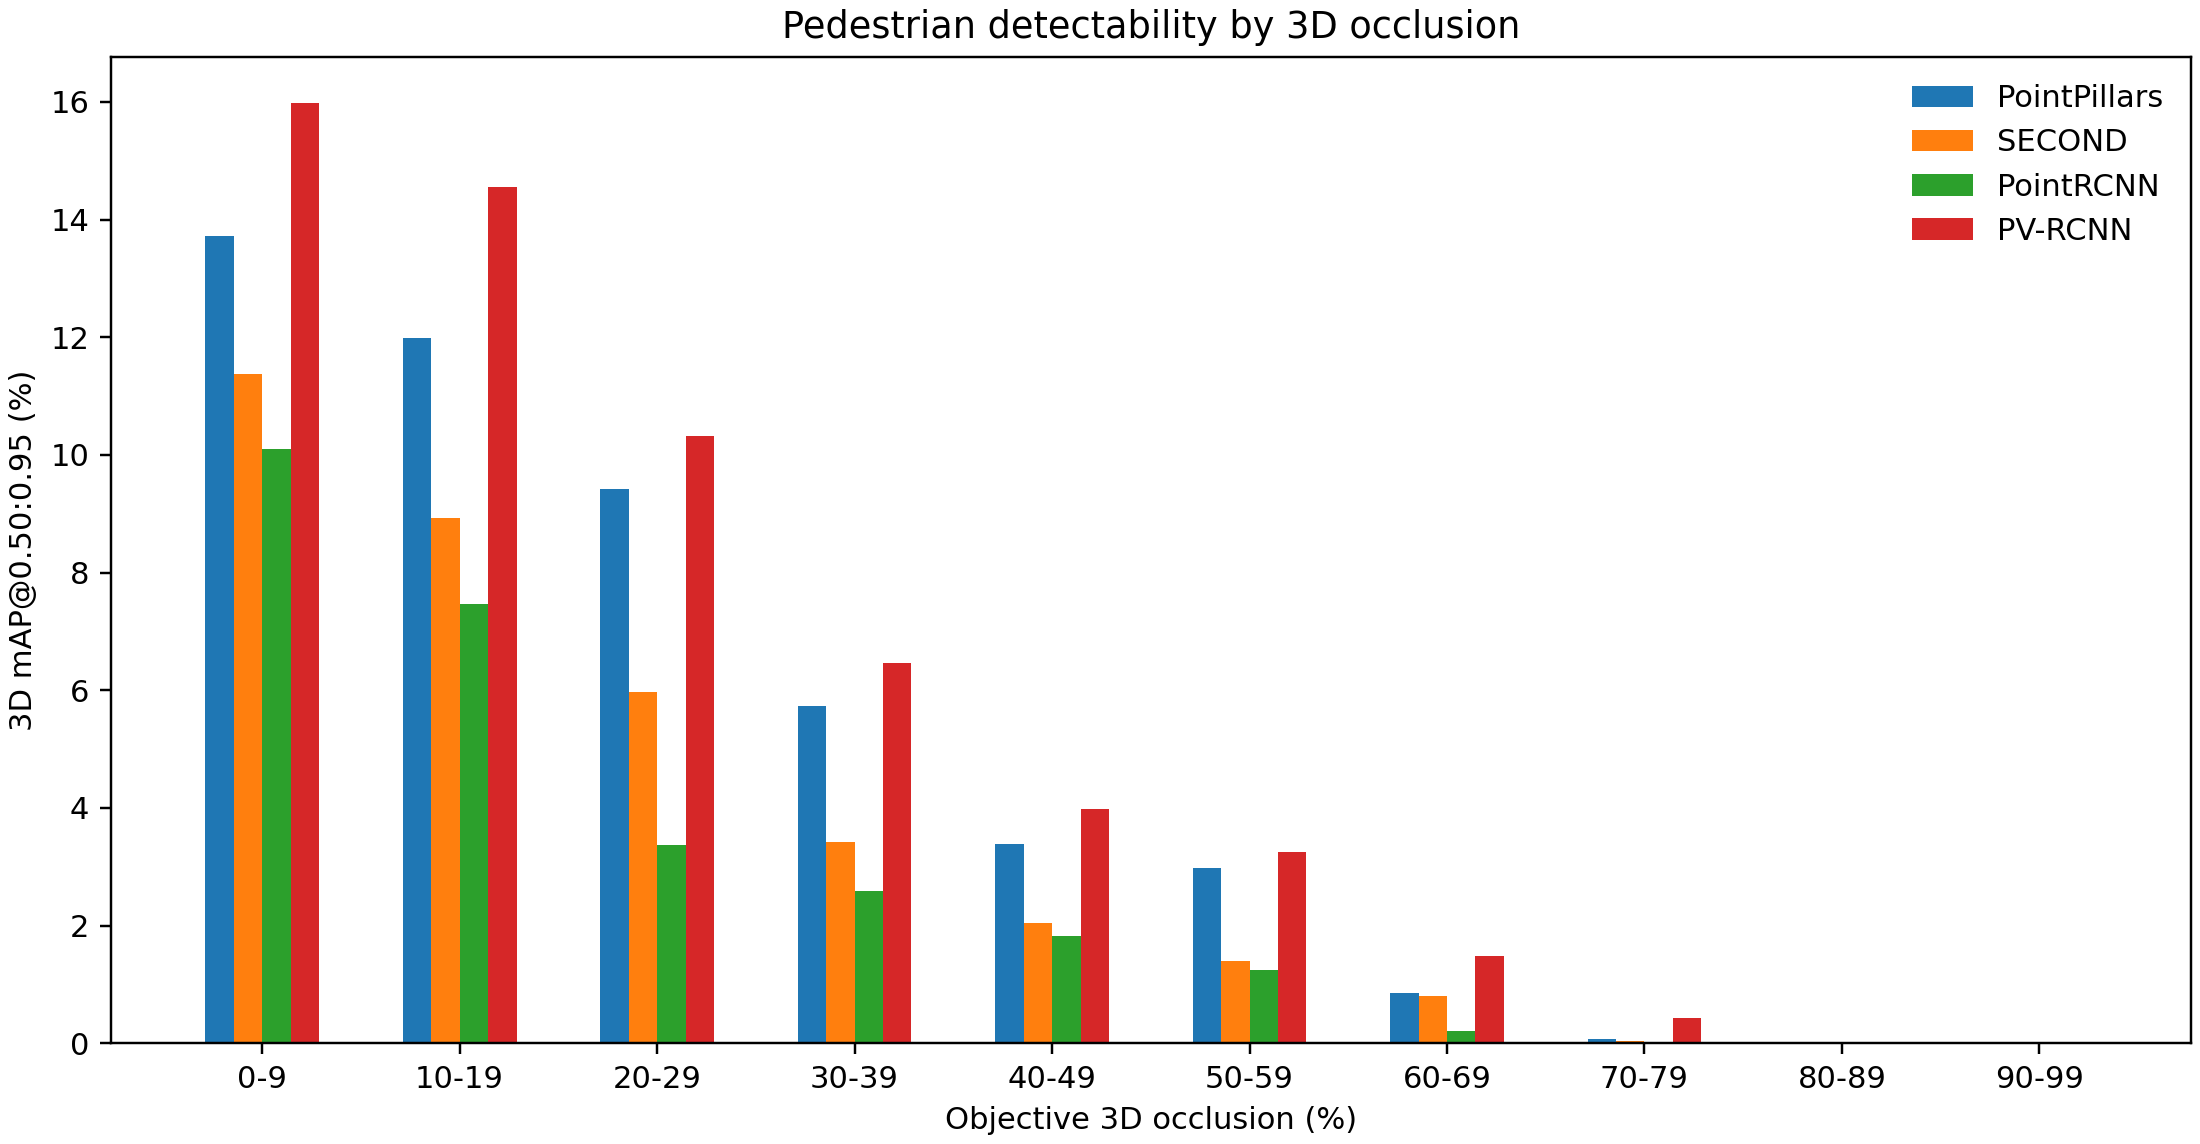
\includegraphics[width=1\linewidth]{images/map-vs-occlusion-baseline.png}
     \caption{mAP vs Occlusion}
     \label{fig:mAP vs Occlusion}
 \end{figure}